\documentclass[a4paper,10pt]{article}
\usepackage{epsfig}
\usepackage{latexsym}
\usepackage{graphicx}
\usepackage{amsfonts}
\usepackage{amsmath}
\usepackage{xcolor}
%\topmargin=-3cm
\topmargin=-1cm
\oddsidemargin=-1cm
\evensidemargin=-1cm
\textwidth=17cm
%\textheight=27cm
\textheight=25cm
\raggedbottom
\sloppy
\title{Polar calibration}
\begin{document}
\section{Quasars results - February 2015}
\subsection{Intensity calibration}
In order to check the calibration we compute the flux of Uranus for each observation done during February 2015. The flux at both wavelengths are consistent with a dispersion of 13$\%$ and 5$\%$ for 1mm and 2mm channel, respectively, see Fig. \ref{photometry}. The expected flux in total power are 38 Jy and 15.93 Jy at 1mm and 2mm respectively. The opacities are shown in Fig. \ref{opacities}.

\begin{figure}[h!]
	 \includegraphics[%
         	width=0.5\linewidth,keepaspectratio]{figures/photometry_Uranus_1mm.pdf}
	 \includegraphics[%
         	width=0.5\linewidth,keepaspectratio]{figures/photometry_Uranus_2mm.pdf}
		\caption{\footnotesize Photometry of Uranus at 1 and 2mm.}
	\label{photometry}
\end{figure}

\begin{figure}[h!]
	\begin{center}
	 \includegraphics[%
         	width=0.5\linewidth,keepaspectratio]{figures/tau_Uranus.pdf}
				\caption{\footnotesize Opacities at 1mm and 2mm.}
	\label{opacities}
	\end{center}
\end{figure}

The same analysis has been done on the observations of the bright quasar 3C84, see the Fig. \ref{photometry_3c84} and Fig. \ref{tau_sed_3C84} for the opacities. The error have been calculated taking into account for the statistical error, 10$\%$ of overall calibration uncertainty, a 2$\%$ of the accuracy for the model used for the estimation of the absolute calibration and 5$\%$ of systematic error introduces by the data reduction filtering. In order to compare with other experiments, we use the data from the Planck and ALMA catalogues, see Fig. \ref{tau_sed_3C84} on right.

\begin{figure}[h!]
	 \includegraphics[%
         	width=0.5\linewidth,keepaspectratio]{figures/photometry_3C84_1mm.pdf}
	 \includegraphics[%
         	width=0.5\linewidth,keepaspectratio]{figures/photometry_3C84_2mm.pdf}
		\caption{\footnotesize Photometry of 3C84 at 1mm and 2mm.}
	\label{photometry_3c84}
\end{figure}

\begin{figure}[h!]
	 \includegraphics[%
         	width=0.5\linewidth,keepaspectratio]{figures/tau_3c84.pdf}
		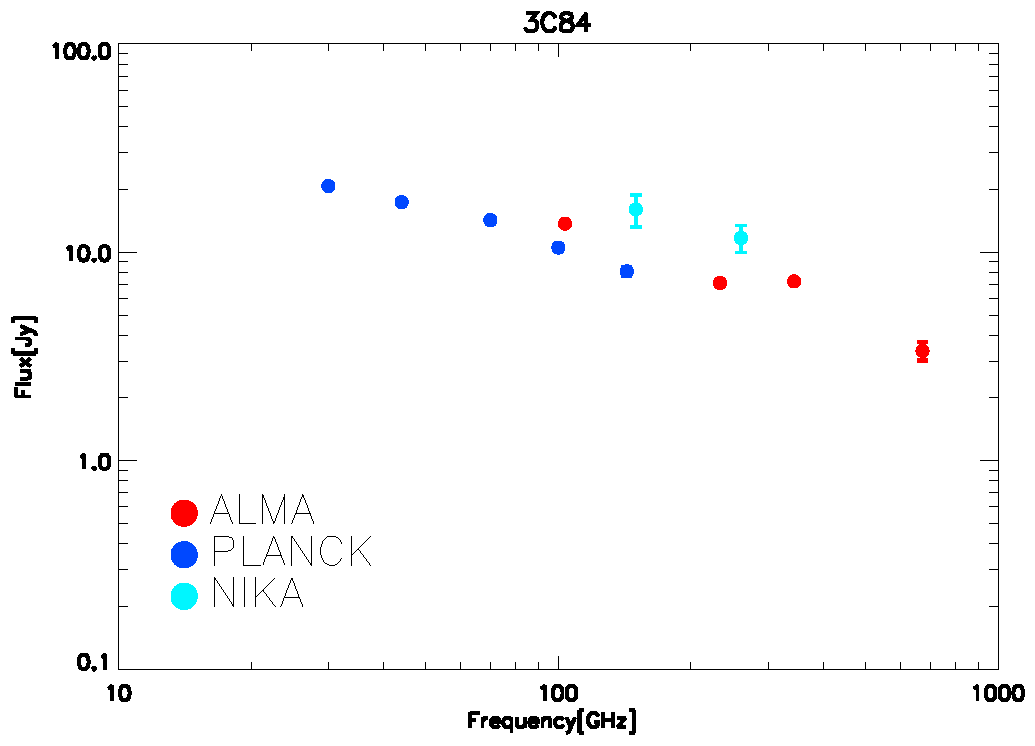
\includegraphics[%
	       width=0.5\linewidth,keepaspectratio]{figures/ALMA_PLANCK_sed_3C84.pdf}
	       		       \caption{\footnotesize Opactities of 3C84 at 1mm and 2mm on left and SED of Planck and NIKA flux in blue on right.}
			       \label{tau_sed_3C84}
\end{figure}


Furthermore, we use the observations of the calibration quasar 3C273 and we do the same analysis discussed above, see the Fig. \ref{photometry_3C273} for the photometry and Fig. \ref{tau_sed_3C273} for the opacities. In the Fig. \ref{tau_sed_3C273} on right the SED of this source using the Planck data.



\begin{figure}[h!]
	 \includegraphics[%
         	width=0.5\linewidth,keepaspectratio]{figures/photometry_3C273_1mm.pdf}
	 \includegraphics[%
         	width=0.5\linewidth,keepaspectratio]{figures/photometry_3C273_2mm.pdf}
		\caption{\footnotesize Photometry of 3C273 at 1mm and 2mm.}
	\label{photometry_3C273}
\end{figure}

\begin{figure}[h!]
	 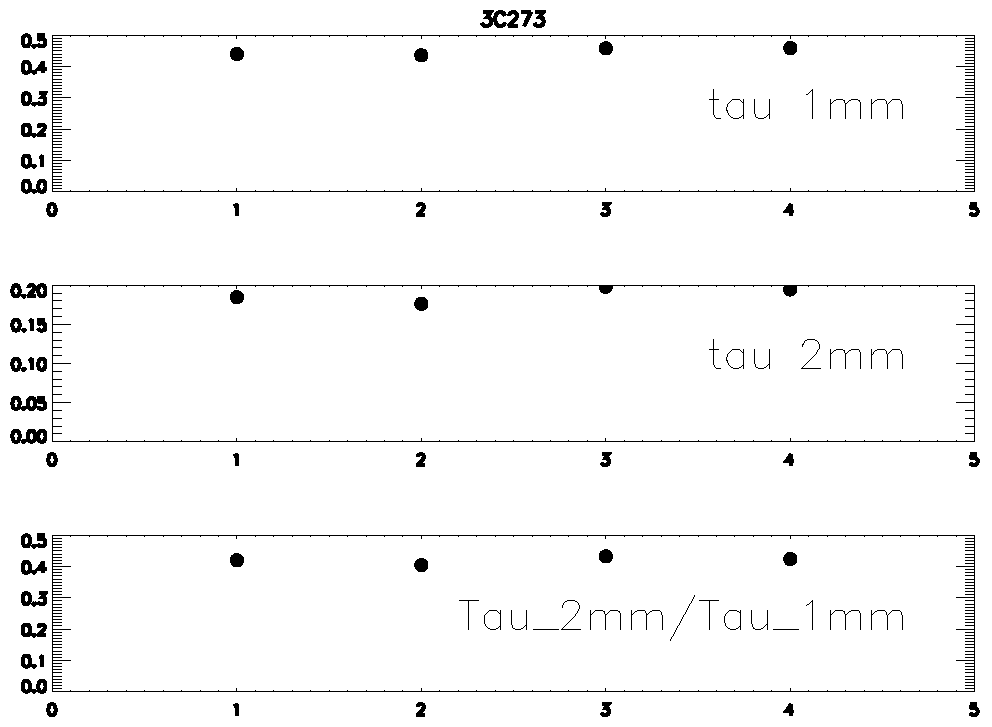
\includegraphics[%
         	width=0.5\linewidth,keepaspectratio]{figures/tau_3C273.pdf}
		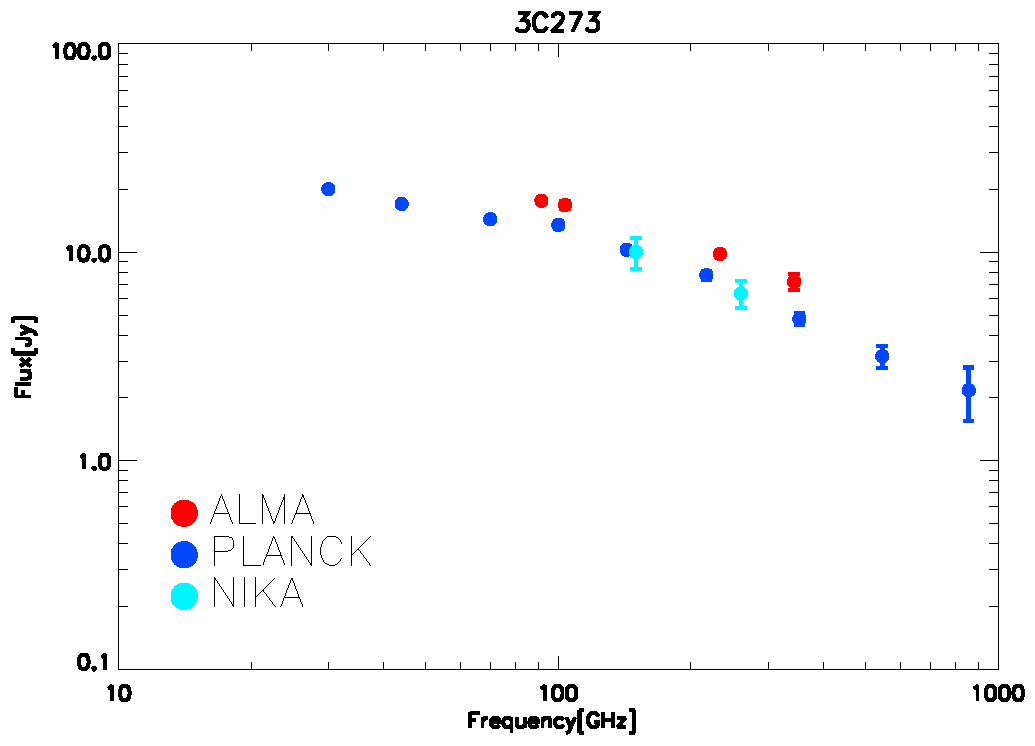
\includegraphics[%
	       width=0.5\linewidth,keepaspectratio]{figures/ALMA_PLANCK_sed_3C273.pdf}
	       		       \caption{\footnotesize Opactities of 3C273 at 1mm and 2mm on left and SED of Planck and NIKA flux in blue on right.}
			       \label{tau_sed_3C273}
\end{figure}


\pagebreak

\section{Polarization of the quasars}
In the tables $\sim$ \ref{tab:tab_quasar_1mm} and \ref{tab:tab_quasar_2mm} we show the results obtained for all quasars observed during the observational campaign in February 2015 at 1.15 mm and 2.05 mm respectively.
The values indicate the flux in intensity and polarisation Q and U, and the consequent polarisation degree p and angle \rm{$\chi$}.

The observations are combined after the pipeline process. This consists of several initial steps for calibration and then, a noise de-correlation, a subtraction of the systematic effect observed on Uranus maps Q and U for each scan in Nasmyth coordinates and a projection in equatorial reference frame. 

The incertitudes in I, Q, U flux values are been calculated fitting a gaussian on several points of each map outside the source region and taking the standard deviation of this collection of fluxes. For the angle we add we take into account for the instrumental incertitude, estimated at 1.8$^\circ$.

For calibration in intensity we compare the parallel observations of NIKA and XPol for the four quasars (3C273, 1749+096, 0851+202, 0415+379) scheduled in table \ref{tab:calib}. The results by the parallel session of the observations by XPol are in tables \ref{tab:xpol_1mm} , \ref{tab:xpol_3mm}, at 1 mm and 3 mm, respectively. 

\begin{table*}[h!]
\caption{Intensity flux by Xpol measurements on February 2015 vs NIKA observations}
\begin{center}
\begin{tabular}{ccccccccc}
\hline
\hline
Source & I flux Xpol 1mm & I flux NIKA 1mm& I flux Xpol 3mm & I flux NIKA 2mm\\
 & [K] & [K] & [K] & [K]\\
\hline
3C273 & 0.614 $\pm$0.002 & 0.60$\pm$ 0.09 &2.304 $\pm$ 0.002 & 1.33$\pm$0.23\\
1749+096 & 0.201$\pm$0.001 & 0.15$\pm$0.03 & 0.558$\pm$0.001 & 0.26$\pm$0.06\\
0851+202 & 0.384$\pm$0.002 & 0.31$\pm$0.06& 0.989$\pm$0.001 & 0.56$\pm$0.13 \\
0415+379 & 0.117$\pm$0.002 & 0.122$\pm$0.025 & 0.343 $\pm$0.000 & 0.235$\pm$0.054\\
\hline
\end{tabular}
\end{center}
\label{tab:calib}
\end{table*}


\begin{table*}[h!]
\caption{Intensity flux, polarisation degree and angle for the quasars observed at 1 mm by XPol}
\begin{center}
\begin{tabular}{ccccccccc}
\hline
\hline
Source & I flux & p & $\chi$ & Comments\\
 & [K] & [\%] & [$^\circ$]\\
\hline
3C273 & 0.614 $\pm$0.002 & 3.6$\pm$ 0.2 & -76.8$\pm$ 1.6 & v\\
1749+096 & 0.201$\pm$0.001 & 2.0$\pm$0.3 & -83.0$\pm$3.7 & vv\\
0851+202 & 0.384$\pm$0.002 & 2.8$\pm$0.3 & -67.5$\pm$2.4 & v\\
0415+379 & 0.117$\pm$0.002 & 2.2$\pm$1.5 & 74.2 $\pm$19.3 & v\\
\hline
\end{tabular}
\end{center}
\label{tab:xpol_1mm}
\end{table*}

\begin{table*}[h!]
\caption{Intensity flux, polarisation degree and angle for the quasars observed at 3 mm by XPol}
\begin{center}
\begin{tabular}{ccccccccc}
\hline
\hline
Source & I flux & p & $\chi$ & Comments\\
 & [K] & [\%] & [$^\circ$]\\
\hline
3C273 & 2.304 $\pm$0.002 & 1.1$\pm$ 0.0 & -37.8$\pm$ 0.9 & flat\\
1749+096 & 0.558$\pm$0.001 & 0.9$\pm$0.1 & 75.0$\pm$1.6 & vv\\
0851+202 & 0.989$\pm$0.001 & 1.1$\pm$0.0 & -38.5$\pm$1.7 & v\\
0415+379 & 0.343$\pm$0.000 & 0.4$\pm$0.1 & -14.2 $\pm$7.2 & v\\
\hline
\end{tabular}
\end{center}
\label{tab:xpol_3mm}
\end{table*}


\subsection{Discussion}
The quasar 3C279 is very variable \cite{lee}, but observations at 350 $\mu$m, 13 mm, 7 mm and 3.5 mm with SHARP polarimeter in the Caltech Submillimeter Observatory on 2014 March show a polarisation degree and angle compatible with our observations. They find an angle $\chi$ = 32$^\circ$-41$^\circ$ at mm wavelengths and p = 10$\%$-12$\%$.

The quasar 3C286 is indicated as a primary calibrator and it has been observed by Xpol \cite{xpol} and recently by CARMA \cite{carma} at 1.3 mm. XPol measures a flux density S$\rm_{3mm}$ = (0.91$\pm$0.02) Jy, a linear polarisation degree p$\rm_{3mm}$ = [13.5 $\pm$ 0.3] $\%$ and a polarisation angle $\chi\rm_{3mm}$ = [37.3$\pm$0.8]$^\circ$. Furthermore, it measures at 1mm a flux density S$\rm_{1mm}$ = [0.30$\pm$0.03] Jy, a polarisation fraction p$\rm_{1mm}$ = [14.4$\pm$1.8] $\%$ and a polarisation angle $\chi\rm_{1mm}$ = [33.1$\pm$5.7]$^\circ$. The quasar 3C286 has been monitored by XPol from 2006 to 2012. It is presented as a calibration source at 3mm and at shorter wavelength. The recently observation at 1.3 mm by CARMA shows an angle $\chi\rm_{1.3mm}$ = [39.2$\pm$1]$^\circ$. These results are in agreement with our observations, see tables \ref{tab:tab_quasar_1mm}, \ref{tab:tab_quasar_2mm}. We compare the flux observed with ALMA and Planck experiments in the Fig. \ref{tau_sed_3C286} on right.

\begin{figure}[h!]
	 \includegraphics[%
         	width=0.5\linewidth,keepaspectratio]{figures/tau_3C286.pdf}
		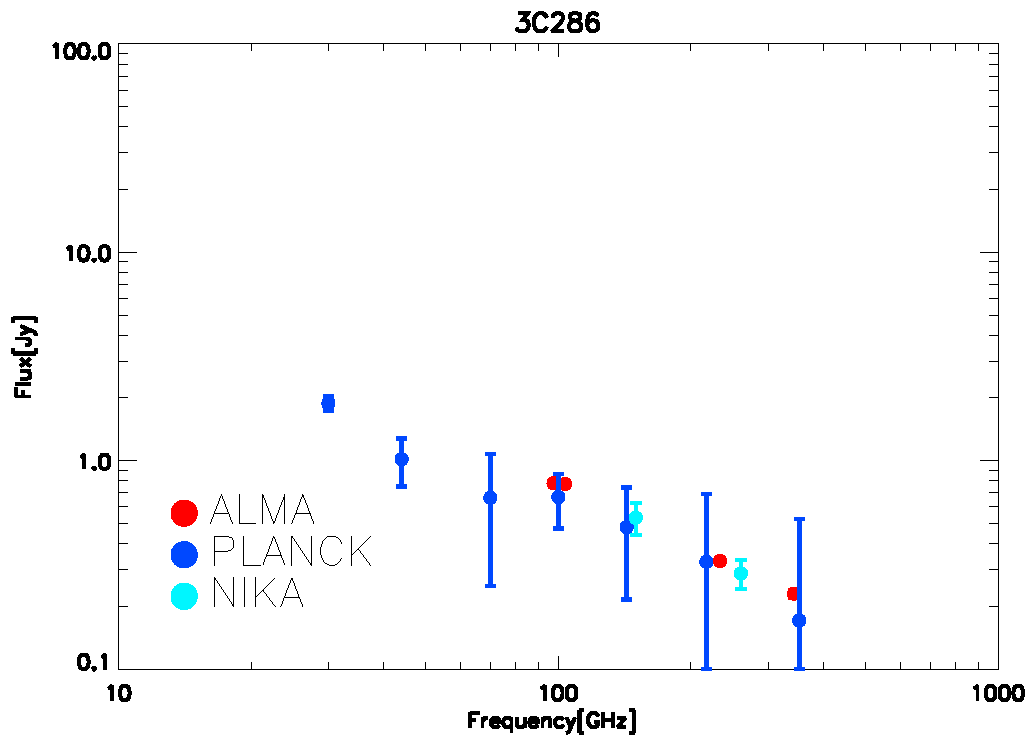
\includegraphics[%
	       width=0.5\linewidth,keepaspectratio]{figures/ALMA_PLANCK_sed_3C286.pdf}
	       		       \caption{\footnotesize Opactities of 3C286 at 1mm and 2mm on left and SED of Planck and NIKA flux in blue on right.}
			       \label{tau_sed_3C286}
\end{figure}


The quasar 3C273 has been observed in parallel with XPol during the campaign on February 2015, the difference in the value of polarisation angle at two wavelength is explained in \cite{jorstad}. %The fig. \ref{3c273} shows the $\lambda^2$ dependence of $\chi$ in 3C 273. There is no unit in the figure and in the text refer to this figure, but I suppose it is in cm$^2$ because of other figures in the paper indicating the same plot for other quasars. You can see the same plots for 3C279 and 0851+202 (OJ 287  in the paper). Anyway, 
Our observations show an agreement with XPol observations at 1mm. 

The quasar 0851+202 is a secondary calibration source, it has a low variability, we don't find an agreement nor with the XPol results or other observations. The expected angle value is negative. 

The quasar 0923+392 is a secondary calibration source and it is detected at 2mm quite well and it is in agreement with previous observations \cite{nartallo}. This paper contains a catalogue of several compact sources.

\subsection{Leakage correction technique}
In the following text we discuss the results obtained using a specific deconvolution/convolution technique to correct for the observed I to Q and U leakage. This technique is more detailed in the appropriate document Polar$\_$leakage$\_$correction that is on svn : Processing/Papers$\_$Proposal$\_$Notes/Notes/Polar$\_$leakage/Polar$\_$leakage$\_$correction.tex.
Using the method described in this document we obtain the following results. 

\begin{table*}[h!]
\caption{Intensity and polarisation fluxes, polarisation degree and angle for the quasars observed at 1.25mm during the campaign on February 2015.}
\begin{center}
\begin{tabular}{ccccccccc}
\hline
\hline
Source & I flux & Q flux &  U flux  & p & $\chi$ & Comments\\
 & [Jy] & [Jy] & [Jy] & [\%] & [$^\circ$]\\
\hline
3C279 &  8.53$\pm$1.7 &  0.25$\pm$0.05 & 0.76$\pm$0.16 & 9.4 $\pm$ 0.7 & 35.8$\pm$2.4 & Very variable (vv)\\
3C273 &  6.35 $\pm$0.9 & -0.25 $\pm$ 0.03 & -0.016 $\pm$0.011 &  3.9$\pm$0.4 & -88.1$\pm$2.9 & parallel session Xpol\\
3C286 &  0.29$\pm$0.05 & 0.021$\pm$0.004 & 0.034$\pm$0.008 & 13.9$\pm$2.43 & 29.0$\pm$4.1 & Calibration source\\
3C345 &  1.08$\pm$0.22 & 0.035$\pm$0.008 & 0.003$\pm$ 0.006 & 3.2$\pm$ 0.4 & 2.7$\pm$ 6.4& (v)no signal in U\\
1749+096 & 1.64$\pm$0.35 & 0.005$\pm$0.005 & 0.06$\pm$0.02 &  3.9$\pm$0.8 & 43.0$\pm$5.1 & (vv) low S/N, no detection Q \\
0851+202 & 3.27$\pm$0.67 & -0.10$\pm$0.02 &  0.02$\pm$0.01 & 3.3$\pm$0.3 & 84.0$\pm$3.84 & no agreement with XPOL\\
0923+392 & 2.04$\pm$0.41 & -0.002 $\pm$0.005 & -0.07 $\pm$ 0.02 & 3.3$\pm$0.5 & -45.78$\pm$4.6 & no signal in Q\\
0415+379 & 1.29$\pm$0.27 & 0.017$\pm$0.009 & -0.025$\pm$0.012 & 2.4$\pm$1.0 &  -28.4$\pm$10.7 &(v) no detection\\
\hline
\end{tabular}
\end{center}
\label{tab:tab_quasar_1mm}
\end{table*}

\begin{table*}[h!]
\caption{Intensity and polarisation fluxes, polarisation degree and angle for the quasars observed at 2.05mm during the campaign on February 2015.}
\begin{center}
\begin{tabular}{ccccccccc}
\hline
\hline
Source & I flux & Q flux &  U flux  & p & $\chi$ & Comments\\
 & [Jy] & [Jy] & [Jy] & [\%] & [$^\circ$]\\
\hline
3C279 &  12.2$\pm$2.8&  0.45$\pm$0.12 &  1.01$\pm$0.24 &  9.2$\pm$ 1.16 & 32.4$\pm$2.9 & Very variable (vv)\\
3C273 & 10.03 $\pm$1.72 & -0.19$\pm$ 0.03 & -0.11$\pm$ 0.02 &  2.24 $\pm$ 0.25 & -74.6 $\pm$ 3.2 & parallel session XPol\\
3C286 & 0.53$\pm$0.09 & 0.037$\pm$0.006 & 0.055$\pm$0.010 & 12.4$\pm$1.6 &  27.7$\pm$3.1 & Calibration source\\\
3C345 &  1.8 $\pm$ 0.4 & 0.03$\pm$0.01 & 0.010$\pm$0.006 & 1.8$\pm$0.4 &  9.2$\pm$5.3\\
1749+096 & 1.98$\pm$0.49 & -0.002$\pm$0.009 & 0.07$\pm$0.02 & 3.6$\pm$0.6 & 45.6$\pm$ 5.2 & Very variable (vv)\\
0851+202 &  4.26$\pm$0.97 & -0.096$\pm$0.023 & 0.079$\pm$0.021 & 2.9 $\pm$ 0.4 & 70.3 $\pm$3.4 & no agreement with Xpol\\
0923+392 & 3.24$\pm$0.75 & -0.016$\pm$0.009 &  -0.087 $\pm$ 0.011 & 2.7$\pm$0.4 & -50.3$\pm$3.9 & agreement\\
0415+379 & 1.77$\pm$0.41 & 0.01$\pm$0.01 & -0.028$\pm$0.007 & 1.7$\pm$0.5 & -34.2$\pm$6.3 & Variable (v) - no detection\\
\hline
\end{tabular}
\end{center}
\label{tab:tab_quasar_2mm}
\end{table*}


%\begin{figure}[h!]
%	\begin{center}
%	 \includegraphics[%
  %       	width=0.5\linewidth,keepaspectratio]{f9.eps}
%		\caption{\footnotesize Dependence of polarisation position angle on square of wavelength in 3C 273. The solid line represents an approximation of the dependence by a $\lambda^2$ Faraday rotation law.}
%	\label{3c273}
%	\end{center}
%\end{figure}
\pagebreak
\section{Crab}
In this section the maps of the Crab nebula obtained after the correction for the systematic effect. The maps are in NASMYTH for now (I have some problem to reproject in RA,DEC).


\begin{figure}[h!]
	 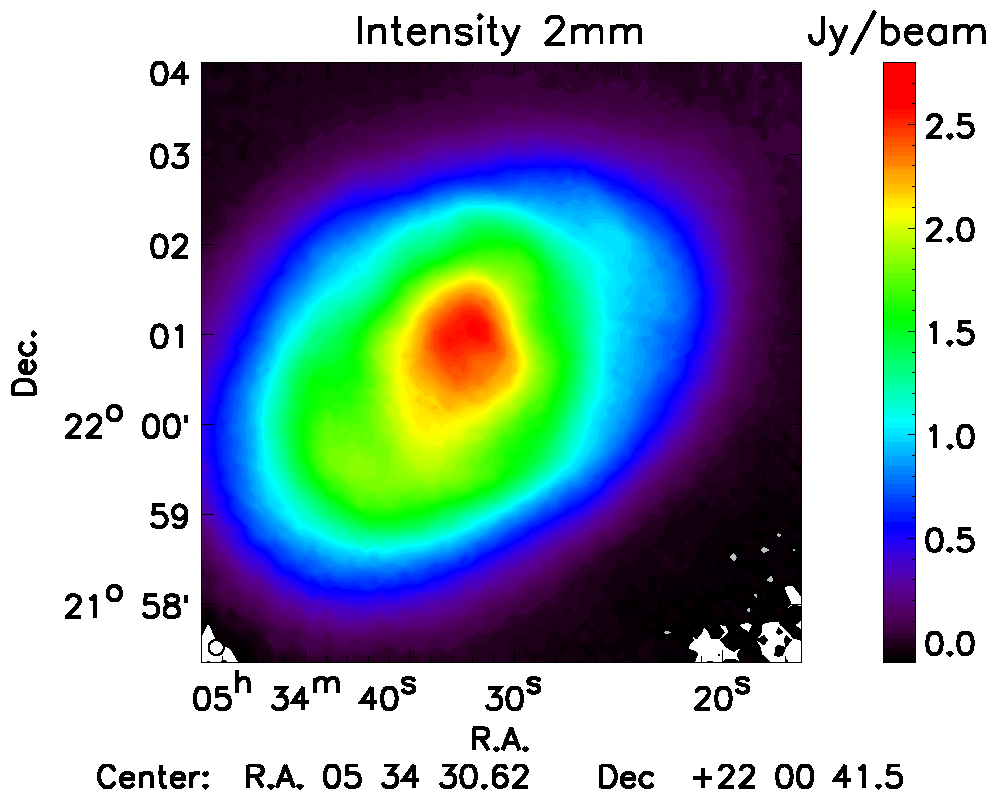
\includegraphics[%
         	width=0.33\linewidth,keepaspectratio]{figures/crab_i_2mm_corrected_nasmyth.pdf}
	  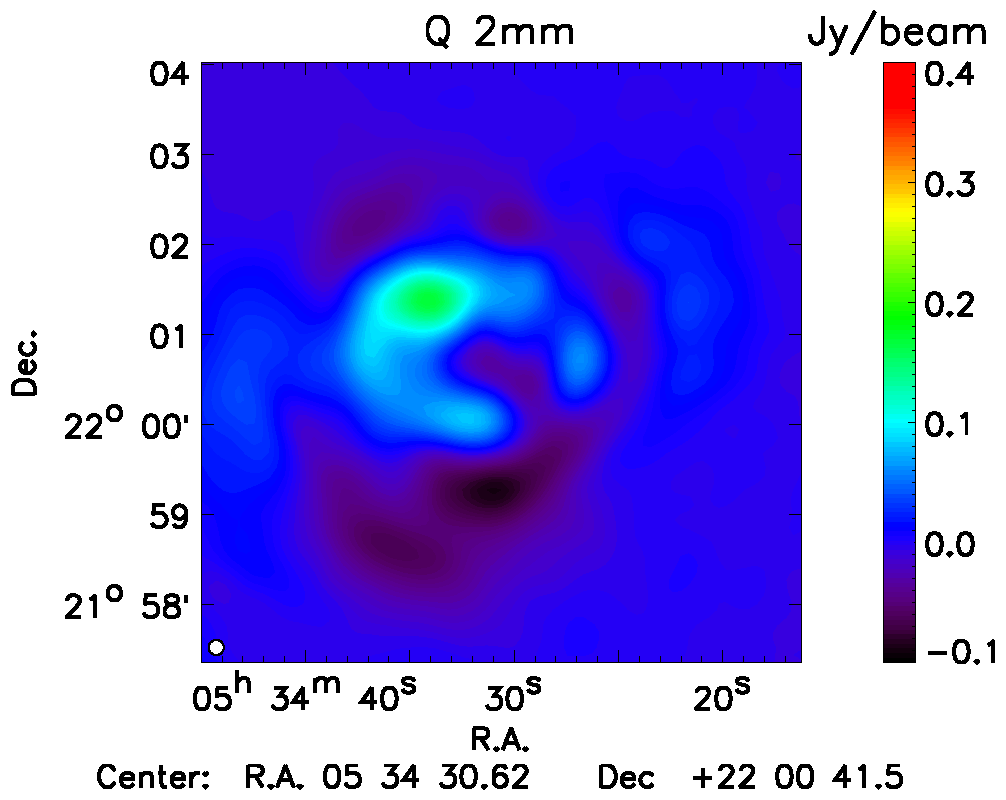
\includegraphics[%
         	width=0.33\linewidth,keepaspectratio]{figures/crab_q_2mm_corrected_nasmyth.pdf}
		  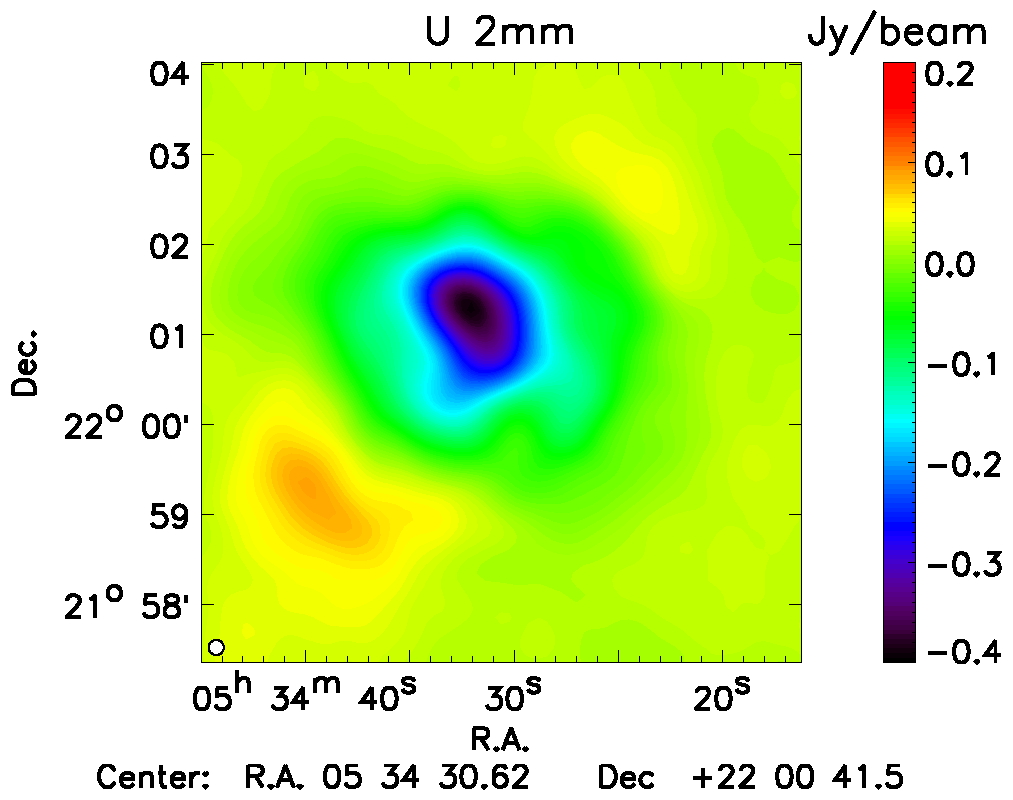
\includegraphics[%
         	width=0.33\linewidth,keepaspectratio]{figures/crab_u_2mm_corrected_nasmyth.pdf}
			
		\caption{\footnotesize Crab nebula maps I, Q, U at 2mm after the correction for the systematic effect. PROJECTION NASMYTH.}
	\label{crab_corrected}
\end{figure}

\begin{figure}[h!]
	 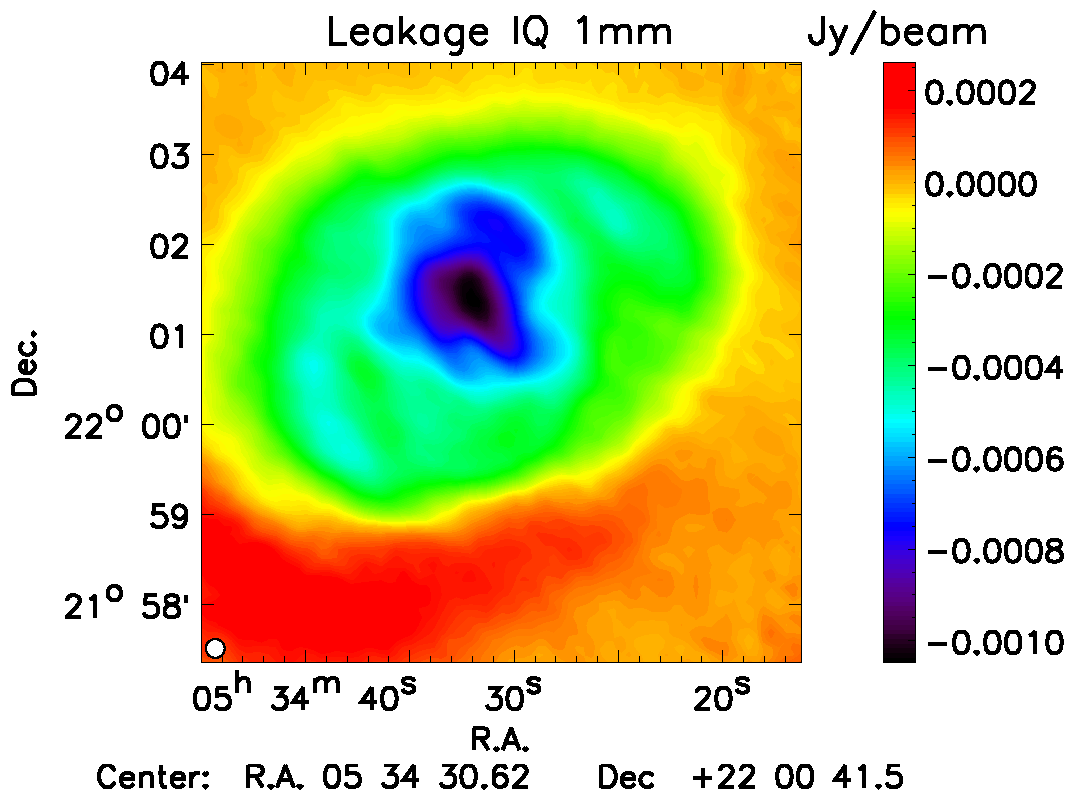
\includegraphics[%
         	width=0.5\linewidth,keepaspectratio]{figures/crab_leakage_q_1mm.pdf}
		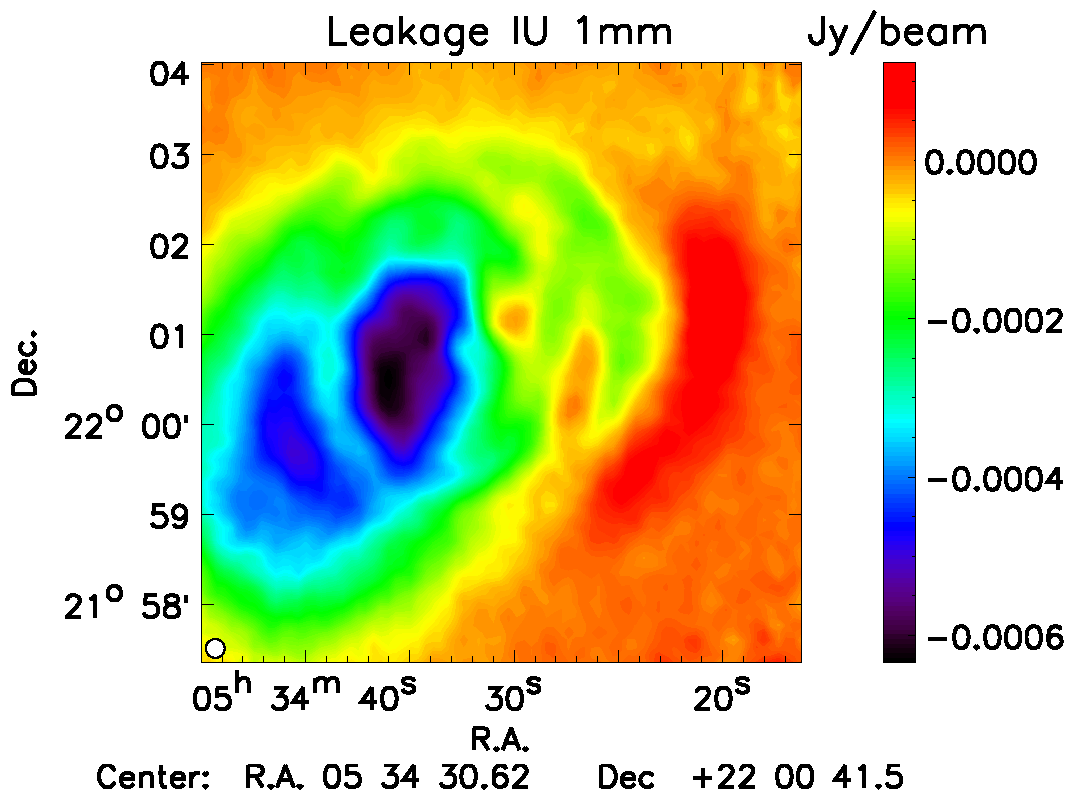
\includegraphics[%
	       width=0.5\linewidth,keepaspectratio]{figures/crab_leakage_u_1mm.pdf}
	       		       \caption{\footnotesize Crab leakage maps IQ, IU at 1mm. }
			       \label{crab_leakage_1mm}
\end{figure}

\begin{figure}[h!]
	 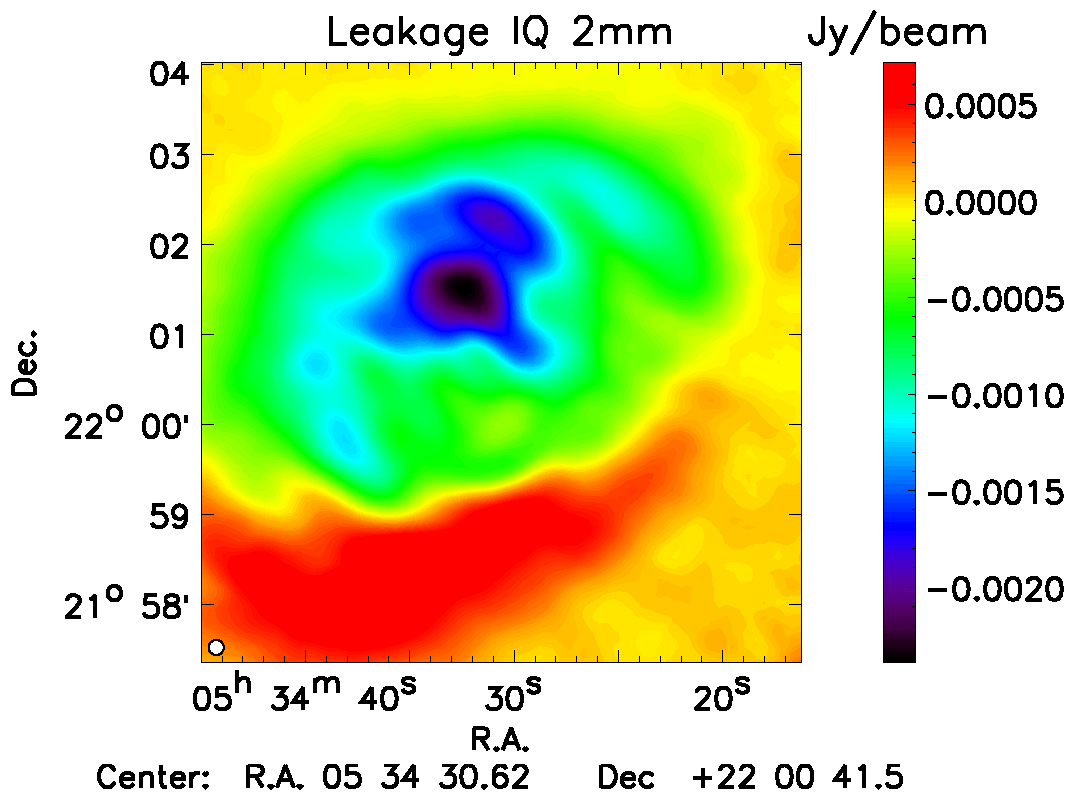
\includegraphics[%
         	width=0.5\linewidth,keepaspectratio]{figures/crab_leakage_q_2mm.pdf}
		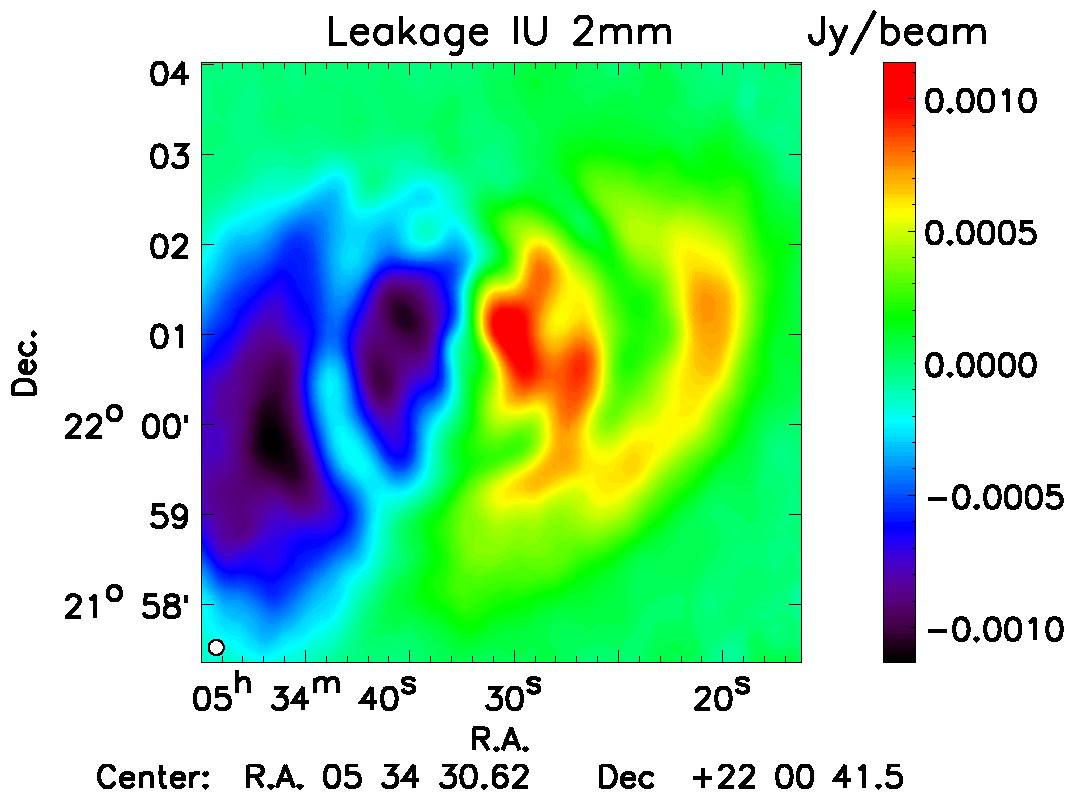
\includegraphics[%
	       width=0.5\linewidth,keepaspectratio]{figures/crab_leakage_u_2mm.pdf}
	       		       \caption{\footnotesize Crab leakage maps IQ, IU at 2mm. }
			       \label{crab_leakage_2mm}
\end{figure}


\pagebreak
\section{Conclusions}
The quasar 3C286 is the primary calibrator and it is in agreement in polarisation degree and angle with previous observations.
The quasar 3C279 is  quite variable but it has been observed recently (2014) and we are in agreement with this observation.
The quasar 3C273 is variable with the wavelength,because of the Faraday rotation. 
The session parallel of XPol experiment confirms our results for the intensity flux.
The leakage effect in the Crab nebula maps is estimated to be $\sim$ 10$^3$.


\pagebreak
\begin{thebibliography}{20}
\bibitem{lee}
Lee, Kang, Byun et al. 2015, "First detection of 350 Micron Polarization From a Radio-loud AGN"
\bibitem{xpol}
Agudo, Thum, Wiesemeyer et al. 2012, "3C 286: a bright, compact, stable, and highly polarised calibrator for millimeter-wavelenght observations"
\bibitem{carma}
Hull and Plambeck 2015, "The 1.3 mm full-stokes polarization system at CARMA"
\bibitem{jorstad}
Jorstad, Marscher, Stevens et al. 2007, "Multiwaveband polarimetric observations of 15 active galactic nuclei at high frequencies: correlated polarisation behavior"
\bibitem{nartallo}
Nartallo, Gear, Murray et al. (printed 2008), "A Millimetre/Submillimetre Polarisation Survey of Compact Flat-Spectrum Radio Sources"

\end{thebibliography}


\end{document}
